% ------------- PREAMBLE ------------- %
% Currently using IEEEtran 1.8
\documentclass[10pt,conference,a4paper]{IEEEtran}

\usepackage[spanish,es-nosectiondot,es-tabla,es-nolists,es-notilde]{babel}
% Intenta corregir los efectos indeseados de babel
\renewcommand{\thesubsection}{\Alph{subsection}}
\renewcommand{\thesubsubsection}{\arabic{subsubsection}}
\addto\extrasspanish{\def\tablename{Tabla}}
\addto\extrasspanish{\def\figurename{Fig.}}

\usepackage{amsmath}
\usepackage{ucs}
\usepackage[utf8x]{inputenc}
\usepackage{times}
\usepackage{graphicx}
\setcounter{MaxMatrixCols}{30}
\usepackage{amsfonts}
\usepackage{amssymb}
\usepackage{url}
\usepackage{epstopdf}
% Style
\newcommand{\CLASSINPUTinnersidemargin}{18mm}
\newcommand{\CLASSINPUToutersidemargin}{12mm}
\newcommand{\CLASSINPUTtoptextmargin}{20mm}
\newcommand{\CLASSINPUTbottomtextmargin}{25mm}
\newcommand{\degree}{\ensuremath{^\circ}}
\DeclareGraphicsExtensions{.png,.eps,.ps,.eps,.jpg}
% Hack para corregir las cabeceras de tablas de IEEEtran. Con esto figuras y tablas tienen el mismo formato.
\makeatletter \def\@IEEEtablestring{} \makeatother

% ------------- DOCUMENT ------------- %
\title{CARACTERIZACIÓN DE MEDIOS DE TRANSMISIÓN}
\author{
    \IEEEauthorblockN{Pablo Arrieta Nata, Daniel Iñigo Baños.}
    \IEEEauthorblockA{uo194468@uniovi.es, uo194823@uniovi.es.}
    \IEEEauthorblockA{Grado en Tecnologias y Servicios de Telecomunicación. Universidad de Oviedo.}
    \IEEEauthorblockA{Sistemas de Telecomunicación. Curso 2013-14.}
}
\begin{document}
\maketitle

\begin{abstract}
    Los medios de transmisión guiados y no guiados, como son el cable coaxial y el canal WiFi, presentan ventajas unos frente a otros en diferentes aspectos. Por esto, dependiendo del tipo de transmisión que se quiera realizar se emplea uno u otro. A continuación se estudian independientemente y se realiza una breve comparación a partir de su análisis en frecuencia.
\end{abstract}

% ------------------------------------------- %
% ------------- PRIMER MONTAJE  ------------- %
% ------------------------------------------- %
\section{Primer Montaje}
Empleando un analizador de redes se mide la respuesta en frecuencia de un cable coaxial mediante el parámetro $s_{2,1}$ en el ancho de banda de 1[MHz] a 2[GHz]. El $s_{2,1}$ representa la función de transferencia del cable en módulo-fase.

A partir de los datos experimentales se mide la atenuación que introduce el cable como $-|H(f)|$ y se compara con los del fabricante (tabla~\ref{tab:atenuacion_coaxial}) y con el modelo teórico según la ecuación~\ref{eq:atenuacion_coaxial}.

Se observa en la figura~\ref{fig:atenuacion_comparada_coaxial} que la atenuación experimental se encuentra entre la que predice el modelo teórico y la que proporciona el fabricante. Esto se debe a que el modelo desprecia muchos factores que influyen en la atenuación y el fabricante trata de dar una cota superior de este añadiendo un margen.
La constante de fase $\beta$, que está modelada por la ecuación~\ref{eq:constante_fase_coaxial}, tiene como pendiente el tiempo de propagación.En la figura~\ref{fig:constante_fase} se ha normalizado el retardo para que las constantes de fase sean comparables.

La respuesta al impulso que se calcula a partir de los datos del analizador de redes es compleja y no causal, por lo que para caracterizar el sistema empleamos $|h(t)| \forall t \geq 0$ representado en la figura~\ref{fig:respuesta_impulso_coaxial}.

La velocidad de propagación por el cable se puede calcular, según la ecuación~\ref{eq:vp_coaxial_experimental}, a partir de la medida del tiempo de propagación, que a su vez se puede obtener de la pendiente de la constante de fase o del instante en que se produce la primera delta de la respuesta al impulso (entre la longitud del cable).
\begin{equation}
    \label{eq:vp_coaxial_experimental}
    v_p [m/s] = \frac{1}{t_d} = \frac{1}{4.55 [ns/m]}
\end{equation}

Según el fabricante la velocidad de propagación es del $66 \%$ de la velocidad de la luz por lo que la $v_p$ se calcularía mediante la ecuación~\ref{eq:vp_coaxial_fabricante} o tomando el valor que aporta directamente en las hojas.
\begin{equation}
    \label{eq:vp_coaxial_fabricante}
    v_p [ms] = 0.66 \cdot 3 \cdot 10^8 [m/s]
\end{equation}

Se puede calcular también mediante la ecuación~\ref{eq:vp_coaxial_modelo} para el cable coaxial. 
\begin{equation}
    \label{eq:vp_coaxial_modelo}
    v_p = \frac{\omega}{\beta} = \frac{1}{\sqrt{\mu \varepsilon}}
\end{equation}.

Como se puede ver en la tabla tiene un error en la velocidad de propagación del $9.88 \%$ respecto al valor del fabricante. 

\subsection{Ecuaciones}

\begin{equation}
    \label{eq:atenuacion_coaxial}
    \alpha = \sqrt{\frac{\rho \omega \epsilon}{2}} \frac{\frac{1}{d_i} + \frac{1}{d_e}}{\ln{\frac{d_e}{d_i}}}
\end{equation}

\begin{equation}
    \label{eq:constante_fase_coaxial}
    \beta = \omega \sqrt{\mu \varepsilon} = \omega \cdot t_d
\end{equation}

\subsection{Figuras y Tablas}

\begin{table}[htb]
    \renewcommand{\arraystretch}{1.2}
    \centering
    \begin{tabular}{|c|c|}
	\hline
	Frecuencia[MHz] & Atenuación [dB/100m] \\
	\hline
	1 & 1.3124 \\
	10 & 4.5934 \\
	50 & 10.8273 \\	
	100 & 16.0769 \\
	200 & 23.9513 \\
	400 & 37.7315 \\
	700 & 55.777 \\
	900 & 65.62 \\
	1000 & 70.5415 \\
	\hline
    \end{tabular}
    \caption{Atenuación en función de la frecuencia que proporciona el fabricante.}
    \label{tab:atenuacion_coaxial}
\end{table}

\begin{table}[htb]
    \renewcommand{\arraystretch}{1.2}
    \centering
    \begin{tabular}{|c|c|}
	\hline
	Fuente & Velocidad de Propagación [m/s] \\
	\hline
	$v_{p fabricante}$ & $198 \cdot 10^6 [m/s]$ \\
	$v_{p experimental }$ & $219.780 \cdot 10^6 [m/s]$ \\
	$v_{p modelo}$ & $198.01 \cdot 10^6 [m/s]$ \\
	\hline
    \end{tabular}
    \caption{Comparación de las velocidades de propagación de la señal por el cable coaxial Belden.}
    \label{tab:vp_coaxial}
\end{table}

\begin{figure}[htb]
    \centering
    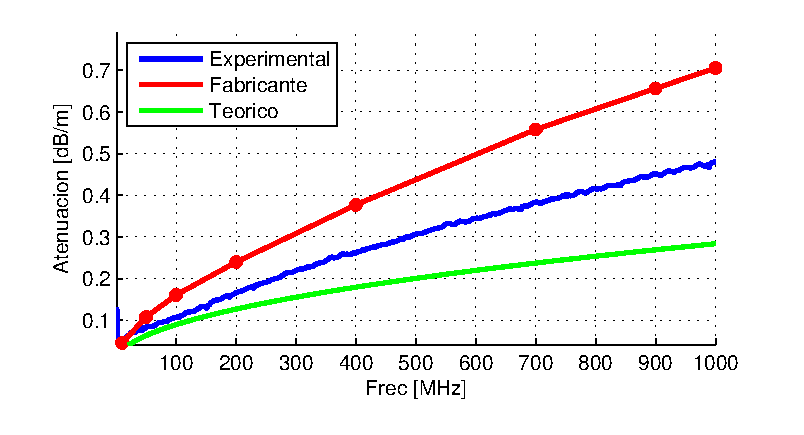
\includegraphics[width=\columnwidth]{figuras/atenuacion_comparada.eps}
    \caption{Atenuación por unidad de longitud en función de la frecuencia en un cable coaxial Belden}
    \label{fig:atenuacion_comparada_coaxial}
\end{figure}
\begin{figure}[htb]
    \centering
    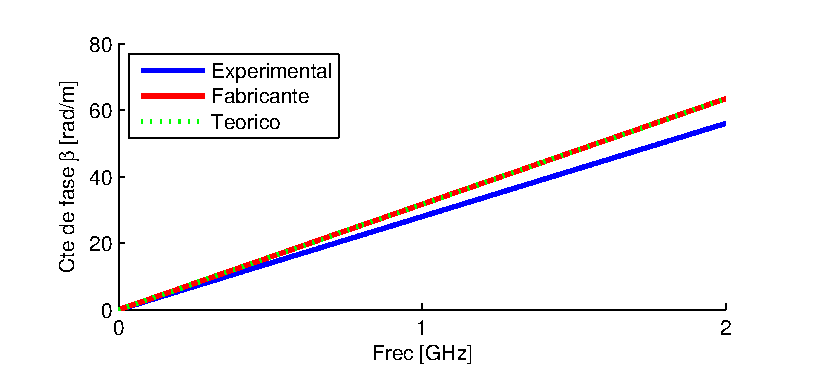
\includegraphics[width=\columnwidth]{figuras/constante_fase.eps}
    \caption{Atenuación por unidad de longitud en función de la frecuencia en un cable coaxial Belden}
    \label{fig:constante_fase}
\end{figure}
\begin{figure}[htb]
    \centering
    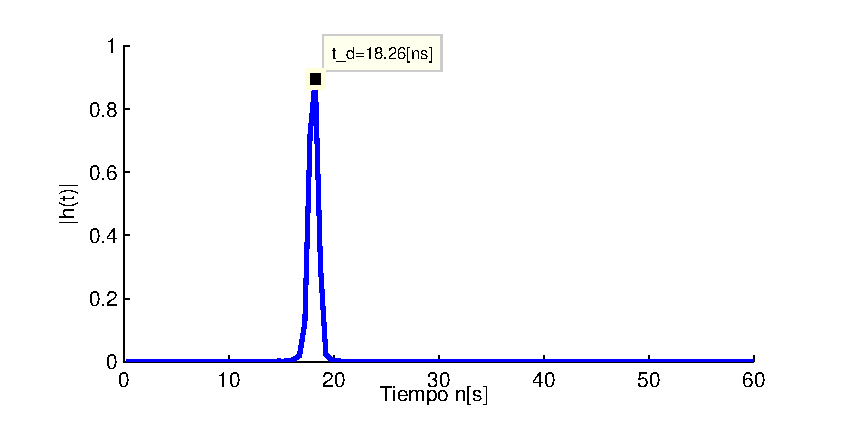
\includegraphics[width=\columnwidth]{figuras/respuesta_impulso.eps}
    \caption{Módulo de la respuesta al impulso del cable Belden de 4[m]}
    \label{fig:respuesta_impulso_coaxial}
\end{figure}
\begin{figure}[htb]
    \centering
    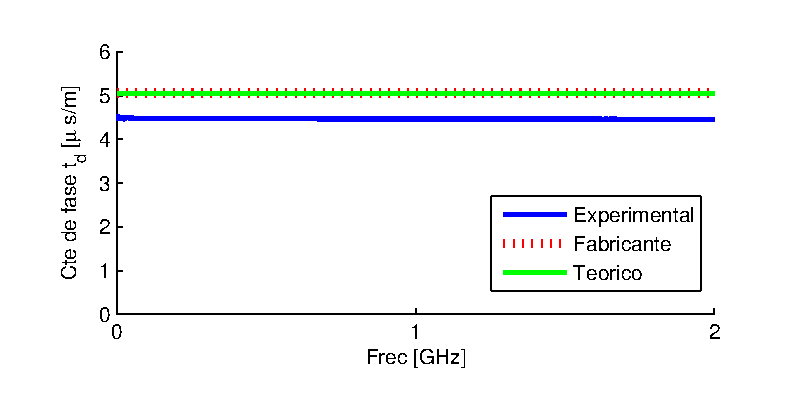
\includegraphics[width=\columnwidth]{figuras/retardo.eps}
    \caption{Atenuación por unidad de longitud en función de la frecuencia en un cable coaxial Belden}
    \label{fig:retardo_coaxial}
\end{figure}

% -------------------------------------------- %
% ------------- SEGUNDO MONTAJE  ------------- %
% -------------------------------------------- %
\section{Segundo Montaje}

Se emplea ahora un medio de transmisión por radiofrecuencia como es el canal WiFi. Su espectro está centrado en $2.4[GHz]$ y los canales tienen un ancho de $20[MH]$. En este caso estudiaremos un solo canal, el que hay en la frecuencia central.Para dar una idea de la $H(f)$ del canal se emplea un $span$ que cubra sólo este. A la hora de analizar el espectro hay que tener en cuenta que no solo estamos midiendo el canal sino que los cables y las antenas también tienen su ganancia y pérdidas.
 
Las medidas sobre la WiFi se realizaron según lo indicado en la figura \ref{fig:posiciones_wifi}. Las medidas son aproximadas siendo $4[m]$ una aproximación de la distancia máxima que permitía el cable que unía la antena móvil con el analizador vectorial de redes.

\begin{itemize}
    \item La primera medida (posición 1 de la figura \ref{fig:posiciones_wifi}) es la más cercana y por lo tanto es la que menos atenuación tiene
    \item La segunda medida se hizo a mas distancia, por lo que la atenuación es algo mayor 
    \item La tercera medida (posición 3 de la figura \ref{fig:posiciones_wifi}) se midió con una placa metálica en paralelo para poder observar el efecto de los ecos. Igualmente al ser un ancho de banda tan pequeño observar ese efecto es difícil porque no tiene porque darse en esas frecuencias
    \item Se realizó una cuarta medida en la misma posición que la tercera pero empleando una polarización horizontal y por lo tanto se observa más atenuación que en la medida anterior
    \item La quinta medida se realizó con un obstáculo (posición 4 de la figura \ref{fig:posiciones_wifi}) que impide la transmisión directa.
\end{itemize}

Luego también se realizaron las medidas para un ancho de $200[MH]$. En este caso se estudia todo el ancho de banda WiFi, con medidas en posiciones análogas a las realizadas para $20[MH]$
\begin{itemize}
    \item La primera medida se realiza a muy corta distancia (posición 1 de la figura \ref{fig:posiciones_wifi}) por lo que en la figura \ref{fig:transferencia_wifi} no se aprecia apenas la atenuación que hay en las bandas de guarda.
    \item La segunda medida se realiza a la máxima distancia que permite el cable pero sin obstáculos. La atenuación es mayor que el caso anterior pero al no haber obstáculos es bastante estable en todo el ancho de banda.
    \item La tercera medida (posición 3 de la figura \ref{fig:posiciones_wifi}) se midió con una placa metálica en paralelo para poder observar el efecto de los ecos. En la figura \ref{fig:transferencia_wifi} se puede observar esos desvanecimientos de manera clara en los picos de atenuación
    \item Se realizó una cuarta medida en la misma posición que la tercera pero empleando una polarización horizontal. Es decir rotando la antena $90\degree$ respecto a la del emisor (o viceversa). La antena WiFi tiene una polarización vertical lineal (según datos del fabricante) y debido a esto la respuesta en frecuencia del canal cae mucho cuando se cambia el plano de polarización. En la figura \ref{fig:transferencia_wifi} podemos observar como tiene una atenuación considerablemente mayor que la medida anterior, también se aprecia que los ecos tienen menos efecto.
    \item La quinta medida se realizó con un obstáculo (posición 4 de la figura \ref{fig:posiciones_wifi}) En esta posición no hay transmisión directa y todo lo que medimos viene dado por ecos y por transmisiones multidireccionales por eso se aprecia la mayor atenuación de todas las medidas y grandes desvanecimientos en valores concretos de la frecuencia.
\end{itemize}

Para calcular el ancho de banda de un canal WiFi lo que tenemos que hacer es medir su potencia central, es decir a $2.4[GHz]$ y luego medir los puntos de frecuencia anterior y posterior donde se registra una perdida de 3dB, la diferencia entre el punto superior e inferior donde encontremos esa perdida es el ancho de banda que se puede asegurar para el canal.



En la figura \ref{fig:respuesta_impulso_wifi} se ve la respuesta al impulso para las diferentes medidas realizadas  un ancho de banda de $200[MH]$
Se aprecian varios picos alrededor del impulso principal que no tienen la misma interpretación para todas las medidas.
\begin{itemize}
    \item En las medidas 1 y 2 estos picos son poco representativos y se acaban alrededor de los 100 ns porque la mayor parte de la transmisión es directa.
    \item En la medida 3 el panel metálico en paralelo nos produce ecos mucho más claros debidos a los rebotes que se producen en este panel nos llevan a que la transmisión multicamino tenga mucha mas relevancia.
    \item La medida 4 se realiza con una polarización horizontal y por tanto los ecos casi no son relevantes porque con esa polarización no se capta suficiente potencia para diferenciarlos
    \item La última medida se realiza con un obstaculo total en medio y por lo tanto es la medida donde los ecos son más perceptibles porque toda la transmision viene dada por ecos y multicamino.
\end{itemize}

En la figura~\ref{fig:transferencia_wifi} se puede observar caida de potencia en las bandas de guarda de los canales en varias f.d.t. a las mismas frecuencias. Aunque no se ve claramente usando solo una, en conjunto se aprecia que el ancho del canal oscila entre 20 y 25[KHz]

\subsection{Figuras y Tablas}
\begin{figure}[htb]
    \centering
    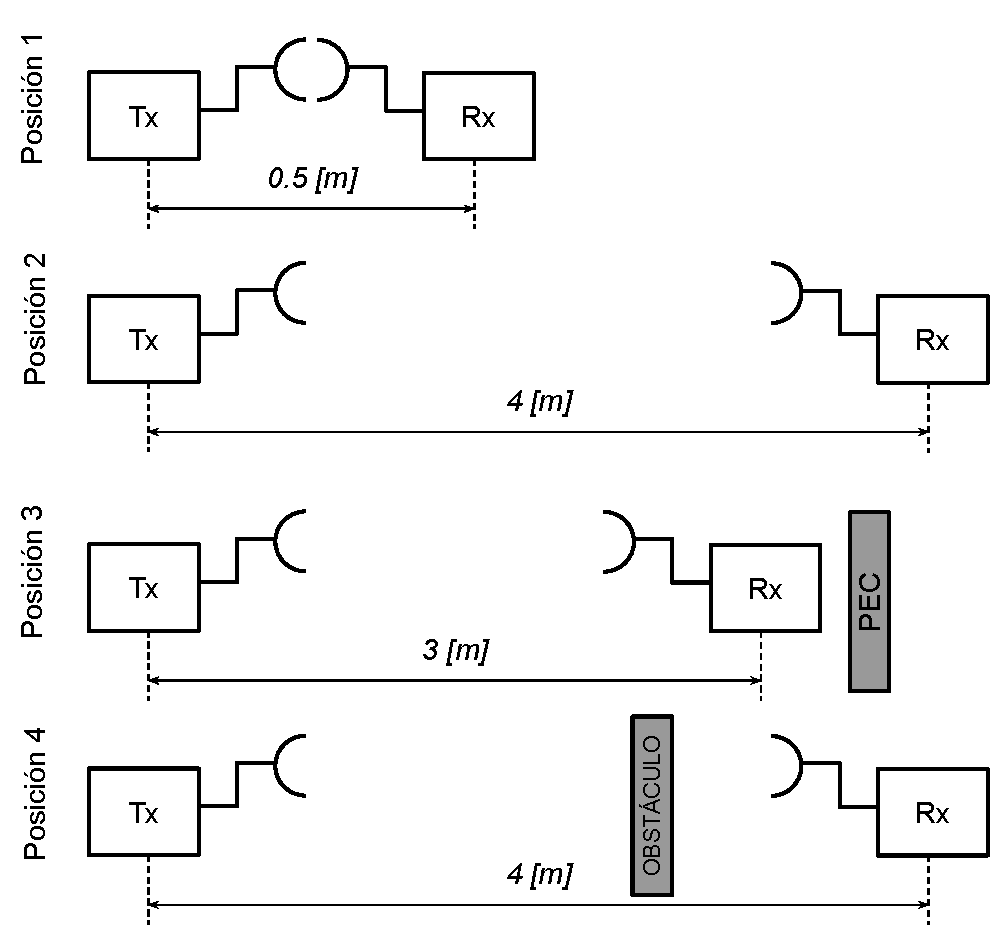
\includegraphics[width=\columnwidth]{figuras/posicion_antenas_wifi.pdf}
    \caption{Topología aproximada para cada medida realizada con las antenas WiFi.}
    \label{fig:posiciones_wifi}
\end{figure}
\begin{figure}[htb]
    \centering
    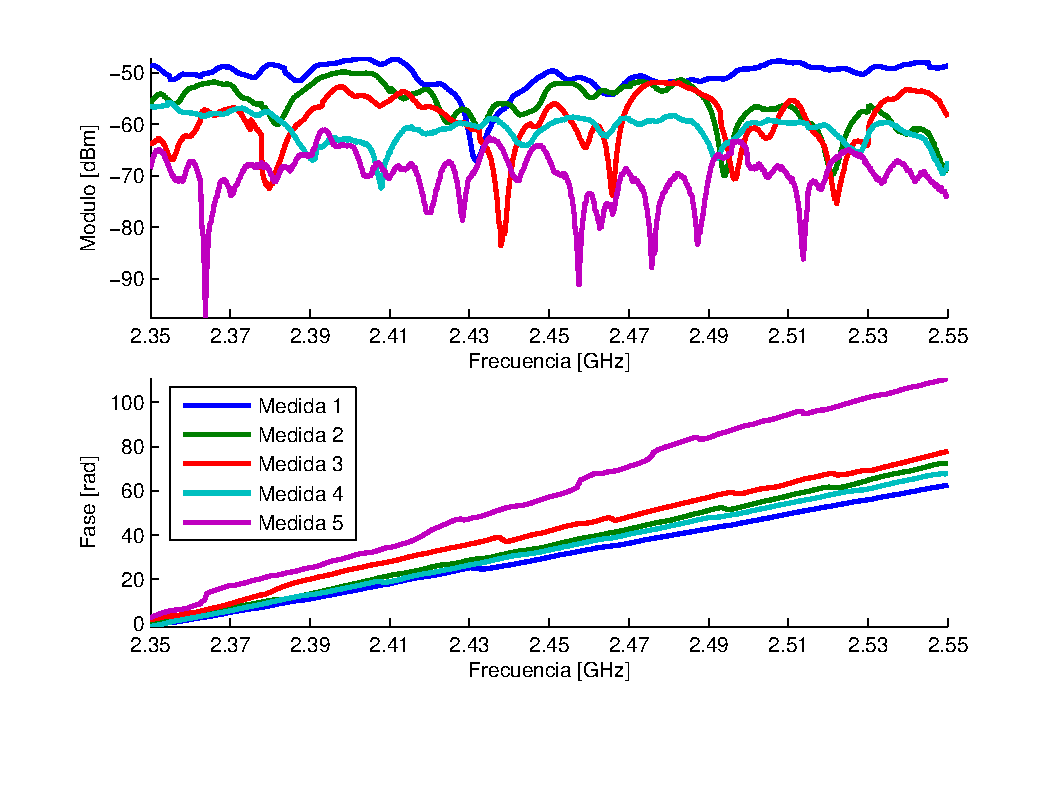
\includegraphics[width=\columnwidth]{figuras/funcion_transferencia_wifi.eps}
    \caption{Función de transferencia del medio wifi con el span de 200[MHz].}
    \label{fig:transferencia_wifi}
\end{figure}
\begin{figure}[htb]
    \centering
    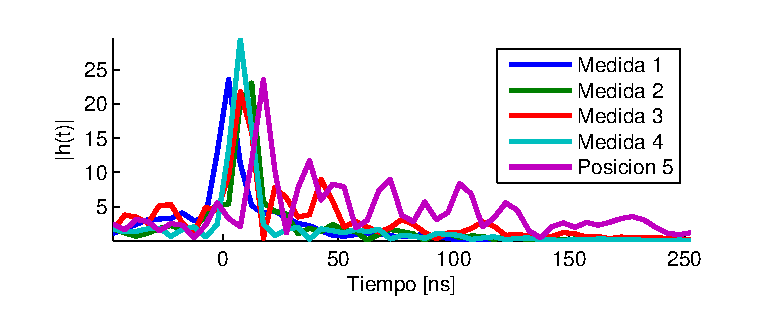
\includegraphics[width=\columnwidth]{figuras/respuesta_impulso_wifi.eps}
    \caption{Respuesta al impulso del WiFi en las diferentes medidas realizadas.}
    \label{fig:respuesta_impulso_wifi}
\end{figure}
%\begin{figure}[htb]
%    \centering
%    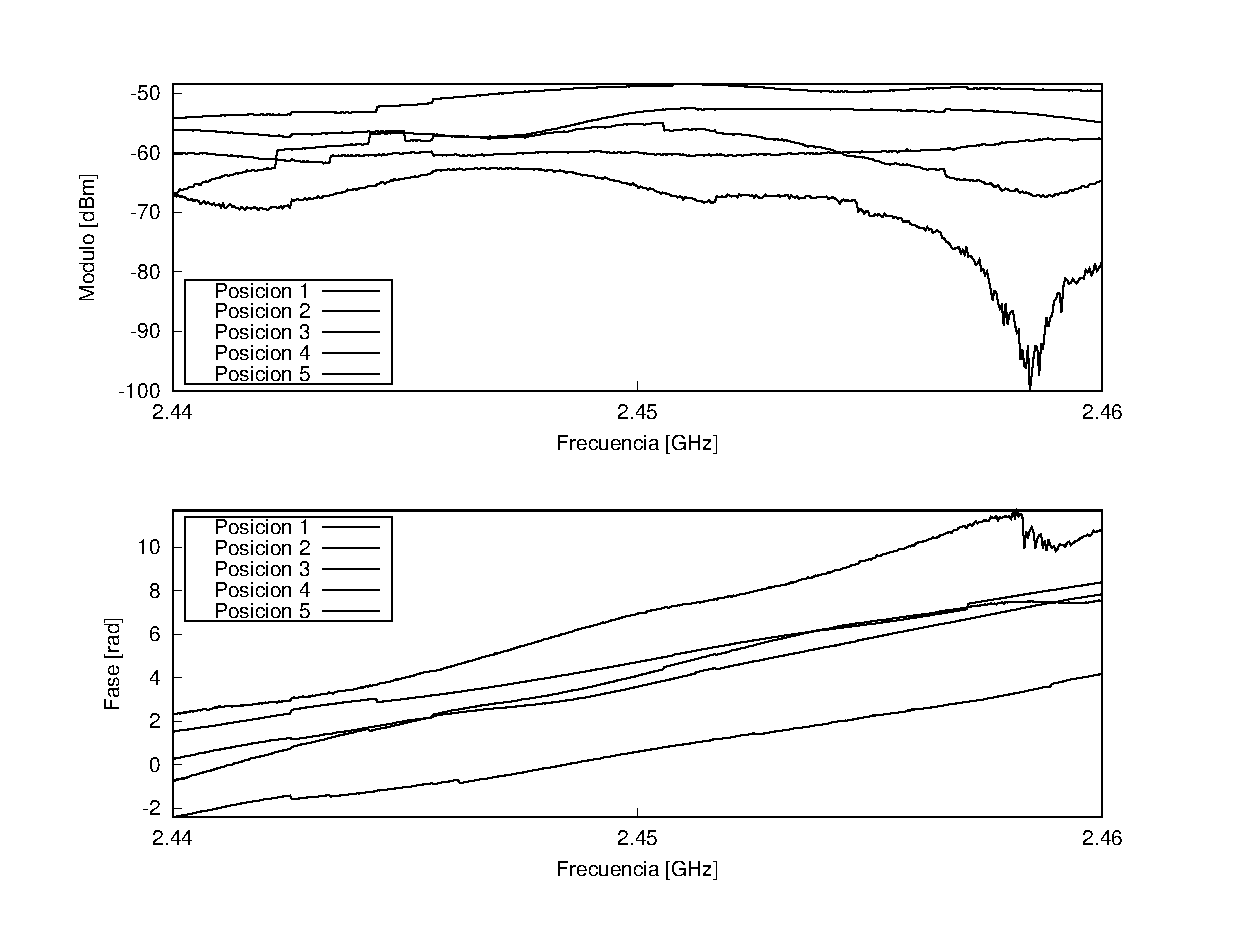
\includegraphics[width=\columnwidth]{figuras/funcion_transferencia_canal_wifi.eps}
%    \caption{Espectro de los canales wifi en cada posición con un span de 20[MHz]}
%    \label{fig:transferencia_canal_wifi}
%\end{figure}
%\begin{figure}[htb]
%    \centering
%    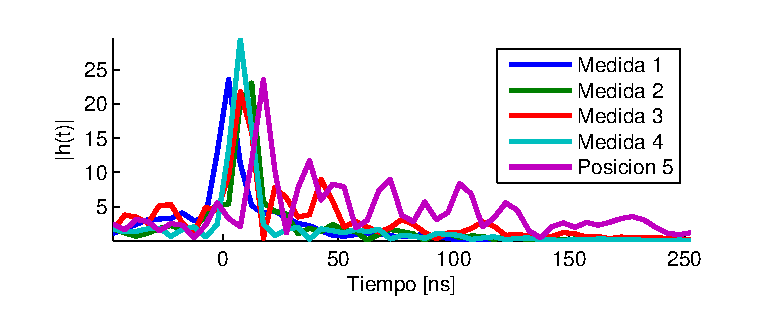
\includegraphics[width=\columnwidth]{figuras/respuesta_impulso_wifi.eps}
%    \caption{Respuesta al impulso del canal wifi en cada posición}
%    \label{fig:impulso_wifi}
%\end{figure}
%\subsection{Ecuaciones}
%\section{Conclusiones}

% ---------------------------------------- %
% ------------- BIBLIOGRAFÍA ------------- %
% ---------------------------------------- %
\newpage
\begin{thebibliography}{2}                                                 %
    \bibitem {ref:libro}Apuntes de Sistemas de Telecomunicación, 2013
    \bibitem {ref:practica}Guión de la práctica de Sistemas de telecomunicación, 2013
\end{thebibliography}

\end{document}
